\chapter{The History On Delegate Approach}
\section{Note}
It is recommended \textbf{not} to skip this chapter, because for the remainder of this book, this book will be making an extensive use of Advanced DL Support library. More information can be found here: https://github.com/Firwood-Software/AdvanceDLSupport

\section{Prior to Nov 2017}
There were at the time that variety of CLR implementations for C\# does not conform to the same behavior expected for P/Invoke. C\# at the time of writing does not have any way to reach the global variable through the normal DllImport attribute approach, and it has to be done by loading libdl and dlopen/dlsym/dlclose. Libdl is a library used to dynamically load external native libraries at runtime and you can retrieve the address to variables or functions by using dlsym which accepts the input for symbol.

In Mono, it would load the external native library with dlopen and you would be sharing the same instance for this external library when using dlopen/dlsym/dlclose. CoreCLR would load the library in other means than dlopen and that would create two instances of the same library which would reflect a different behavior.
\newpage
\section{Precursor to Advanced DL Support}
ADL, Advanced DL Support, was created shortly after Nov 2017 to work around the problem with P/Invoke and inconsistent behavior with different implementations of CLR. It was initially accomplished by doing the followings in concept:

\lstinputlisting[style=customcs]{codes/Chap4/Chap4Snippet1.cs}

But this is an extremely inefficient approach to wrap native libraries. Advanced DL Support utilizes CIL, Common Intermediate Language, the language that C\# compiles to, to generate new types and return new instances of said types for you to utilize native libraries which can be disposed, and therefore do no longer have to be kept around for the duration of the program runtime. You can create new types and code while the program is running and that is thank to the Just-In-Time Compiler. You supplement an interface, abstract class or even a base class to ADL to generate a new type at runtime that binds all of the functions and variables and make it significantly easier to bind native library at an equivalent speed to DllImport attribute approach.

\newpage
\section{The Advanced DL Support Approach}
Make sure you have a new directory created for Chapter 4 and run the following to initialize your Dotnet Console project:

\lstinputlisting[style=custombash, language=C]{codes/Chap4/Chap4Snippet2.sh}

We will need to both reference ''AdvancedDLSupport'' from Nuget and to add compilation target for C Library that we will be wrapping with for this demonstration.

Your CsProj file should looks like this:

\lstinputlisting[style=customxml, language=XML]{codes/Chap4/Chap4Snippet3.xml}

The C Library source could will simply have a global variable and a function to increment the said variable as followed:

\lstinputlisting[style=customc, language=C]{codes/Chap4/Chap4Snippet4.c}

For demonstration of ADL, the native library can be binded in C\# by simply creating an interface for library and it supports properties:

\lstinputlisting[style=customcs]{codes/Chap4/Chap4Snippet5.cs}
\newpage
The following output from the program will display as followed:

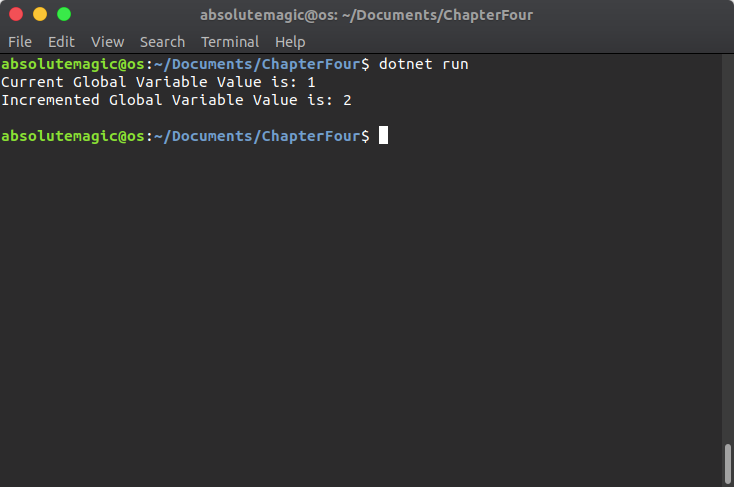
\includegraphics[width=\textwidth]{ChapterFourConsole}

As you can tell, the amount of time saved in writing the binding for native library compared to both DllImport and the Delegate Approach are very significant. You simply only have to write an interface to the native library and that eliminates the need for writing DllImport attribute repeatingly and you can also access the global variable via properties.
